\title{Midterm Solutions for Electromagnetic Theory (PHYS330)}
\author{Dr. Jordan Hanson - Whittier College Dept. of Physics and Astronomy}
\date{\today}
\documentclass[10pt]{article}
\usepackage[a4paper, total={18cm, 27cm}]{geometry}
\usepackage{amsmath}
\usepackage{graphicx}
\usepackage{hyperref}

\def\rcurs{{\mbox{$\resizebox{.16in}{.08in}{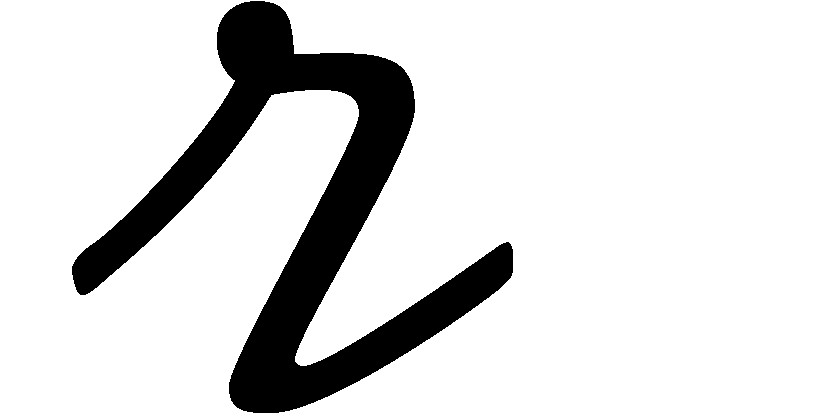
\includegraphics{ScriptR}}$}}}
\def\brcurs{{\mbox{$\resizebox{.16in}{.08in}{
\includegraphics{BoldR}}$}}}
\def\hrcurs{{\mbox{$\hat \rcurs$}}}

\begin{document}
\maketitle

\begin{abstract}
This exam may be completed at home, and covers chapters 1-3 of the course text and in-class examples.  Class notes and the course text may be used (open book), but no internet sources are allowed.  The daily warm-up exercises are good study materials for this exam.
\end{abstract}
\noindent

\section{Math Bootcamp}

\begin{enumerate}
\item (a) If $\mathbf{A}$ and $\mathbf{B}$ are two vector functions, what does the expression $(\mathbf{A} \cdot \nabla) \mathbf{B}$ mean?  That is, what are its $x$, $y$, and $z$ components, in terms of the Cartesian components of $\mathbf{A}$, $\nabla$, and $\mathbf{B}$? (b) Compute $(\hat{r} \cdot \nabla) \hat{r}$, where $\hat{r}$ is $\mathbf{r}/r$. (c) One can show that the \textit{force} on a dipole induced by a non-uniform field is
\begin{equation}
\mathbf{F} = (\mathbf{p} \cdot \nabla) \mathbf{E}
\end{equation}
Compute the force on a physical dipole located at the origin with $\mathbf{p} = q \mathbf{d} = qd~\mathbf{\hat{x}}$ in a field with associated potential $V(\mathbf{r}) = V_0 r^2 + V_1$. \\
\begin{itemize}
\item (a) $(\mathbf{A}\cdot\nabla)\mathbf{B} = A_x \frac{\partial\vec{B}}{\partial x} + A_y \frac{\partial\vec{B}}{\partial y} + A_z \frac{\partial\vec{B}}{\partial z}$
\item (b) $(\hat{\mathbf{r}} \cdot \nabla)\hat{\mathbf{r}} = \mathbf{0}$
\item (c) $\mathbf{F} = -2 V_0 \mathbf{p}$.  The units are equivalent to $q E$, a force.  The direction makes sense if you visualize the dipole in a bowl-shaped potential (negative charge rolls uphill).  The potential is a bowl-shape to first-order.
\end{itemize}
\item Evaluate the following integral using (a) the three-dimensional Dirac delta function, or (b) integration by parts.  Solving both earns a bonus point.
\begin{equation}
J = \int_{\mathcal{V}} e^{-r} \left( \nabla \cdot \frac{\mathbf{\hat{r}}}{r^2} \right)
\end{equation} \\ 
\begin{itemize}
\item (a) The integral is equivalent to evaluating the integrand at the origin, since it involves the Diract delta-function in three dimensions.
\begin{equation}
J = \int_\mathcal{V} e^{-r} 4\pi \delta^3(\mathbf{r}) d\tau' = 4\pi
\end{equation}
\item (b) Integration by parts, taking the surface and volume corresponding to a sphere of radius $R$:
\begin{align}
e^{-r} \left( \nabla \cdot \frac{\hat{r}}{r^2} \right) &= \nabla \cdot \left(e^{-r} \frac{\hat{r}}{r^2}\right) + \frac{e^{-r}}{r^2} \\
J &= \oint_\mathcal{S} e^{-r} r^{-2} \hat{r} \cdot d\mathbf{a} + \int_\mathcal{V} \frac{e^{-r}}{r^2}d\tau' \\
J &= 4\pi \left(e^{-R} R^{-1} + \left.e^{-r}\right|_R^0 \right), ~~ R \to \infty \\
J &= 4\pi
\end{align}
Thus the two methods give the same answer.
\end{itemize}
\end{enumerate}

\clearpage

\section{Electrostatics}

\begin{enumerate}
\item Suppose two dipoles, each with dipole moment $\mathbf{p}$ pointed in opposite directions, form a square with alternating positive and negative charges and side length $d$.  Calculate the field $\mathbf{E}_{\rm tot}$ at the following points $P$: (a) $P = (0,0)$, (b) $P = (2d,0)$, and $P = (0,2d)$.  Check units and take limits\footnote{This object is an electrostatic quadrupole.}.  \\ 
\begin{itemize}
\item (a) $\mathbf{E} = \mathbf{0}$, by symmetry.
\item (b) Break the problem into pieces, assuming $+q$'s are in first and third quadrants, and $-q$'s are in the second and fourth quadrants:
\begin{align}
\mathbf{E} &= \sum_i \frac{k q_i}{\rcurs_i^2}\hrcurs_i = kq\left(\frac{\hrcurs_1}{\rcurs_1^2} - \frac{\hrcurs_2}{\rcurs_2^2} + \frac{\hrcurs_3}{\rcurs_3^2} - \frac{\hrcurs_4}{\rcurs_4^2}\right) \\
\hrcurs_{1,2} &= \left(3\sqrt{2}\hat{x} \mp \sqrt{2}\hat{y}\right)/\sqrt{20} \\
\hrcurs_{3,4} &= \left(\sqrt{25}\hat{x} \pm \hat{y}\right)/\sqrt{26} \\
\rcurs_{1,2}^2 &= \frac{5}{2}d^2 \\ 
\rcurs_{3,4}^2 &= \frac{13}{2}d^2 \\ 
\end{align}
\item Note that summing the four contributions eliminates the $\hat{x}$ components.  This is expected from symmetry considerations:
\begin{equation}
\mathbf{E} = \frac{4kq}{d^2}\hat{y} \left( \frac{1}{13\sqrt{26}} - \frac{\sqrt{10}}{25}\right) \approx -\frac{4kq}{9d^2}\hat{y}
\end{equation}
\item (c) By symmetry, \textbf{the field should be identical}, except in the $-\hat{x}$ direction.
\end{itemize}
\item The electric potential of some configuration is given by the expression
\begin{equation}
V(\mathbf{r}) = A \frac{e^{-\lambda r}}{r} \label{eq:lambda}
\end{equation}
In Eq. \ref{eq:lambda}, $A$ and $\lambda$ are constants.  Find the field $\mathbf{E}(\mathbf{r})$, the charge density $\rho$ and the total charge $Q$ in terms of $A$ and $\lambda$.  \textit{Hint: $\rho = \epsilon_0 A(4\pi\delta^3(\mathbf{r}) - \lambda^2\exp(-\lambda r)/r)$.} \textbf{Bonus:} compute the total energy stored in the field over all space. \\
\begin{itemize}
\item (a) The gradient leads to the $\mathbf{E}$-field, and just the $\hat{\mathbf{r}}$-component is necessary:
\begin{equation}
\mathbf{E} = A\hat{\mathbf{r}} \left( \frac{e^{-\lambda r}}{r^2} + \frac{\lambda e^{-\lambda r}}{r} \right)
\end{equation}
\item Note that, by Gauss' Law, $\rho = \epsilon_0 \nabla \cdot \mathbf{E}$.  Taking the appropriate derivatives leads to 
\begin{equation}
\rho = -\epsilon_0 A \lambda^2 \frac{e^{-\lambda r}}{r}
\end{equation}
The trouble is when $r = 0$, and Problem 1.2 should be a clue.  The divergence \textit{itself} blows up as $r \to 0$, so we should first take the limit of $\mathbf{E}$ as $r \to 0$.  The result is (to lowest order):
\begin{equation}
\mathbf{E} = A\hat{\mathbf{r}} r^{-2} \label{eq:div}
\end{equation}
And when we take the divergence of Eq. \ref{eq:div}, we encounter the three-dimensional Dirac $\delta$-function.  Collecting the results together gives
\begin{equation}
\rho = \epsilon_0 A \left( 4\pi\delta^3(\mathbf{r}) - \frac{\lambda^2 e^{-\lambda r}}{r}\right)
\end{equation}
The units check out because $\epsilon_0 A$ has units of Coulombs, and $A$ has units of Volt-meters.
\item The total charge is the volume integral of $\rho$, and the results \textit{turns out to be zero.}  This is a highly intriguing result, because it must describe something about a spherically symmetry atomic structure with a positive center and negative outer shell, or a \textit{shielded} positive charge with overall neutrality.
\item \textbf{Bonus:} Given that there is a Dirac $\delta$-function in the charge density, the energy density should diverge if we include the origin.  This can be checked numerically, and represents a good final project idea.
\end{itemize}
\item (a) Use Gauss' Law to compute the field $\mathbf{E}$ as a function of the distance $s$ from a long straight wire with positive charge density $\lambda$. (b) Calculate the position versus time of a positive point charge $q$ with mass $m$ if it is released a distance $s$ from the wire. \\ \\
Using Gauss' Law, we can show that the field is
\begin{equation}
\mathbf{E} = \frac{\lambda}{2\pi\epsilon_0 s}\hat{s}
\end{equation}
Newton's 2nd law tells us that
\begin{align}
\frac{d^2 s}{dt^2} &= \frac{C}{s} \label{eq:diff} \\
C &= \frac{q}{m}\frac{\lambda}{2\pi\epsilon_0}
\end{align}
Note that the constant $C$ has units of acceleration times distance.  This is a rather difficult differential equation.  What if we assume that $s(t)$ is a power series, and take it to quadratic order in $t$?  This would treat the acceleration as a constant, which is not inaccurate, due to the shape of the field.  All the acceleration occurs \textit{near} the charge distribution, and weakens as the particle moves away.  Let
\begin{equation}
s(t) = \sum_{n = 0}^{\infty} a_n t^n \approx a_0 + a_1 t + a_2 t^2
\end{equation}
Note that Eq. \ref{eq:diff} simplifies to
\begin{equation}
s \frac{d^2 s}{dt^2} = 2 a_2 (a_0 + a_1 t + a_2 t^2) = C
\end{equation}
Boundary conditions:
\begin{itemize}
\item At $t=0$, $s = s_i$, the initial position $\rightarrow a_0 = s_i$
\item At $t = 0$, $ds/dt = 0$, zero initial velocity, and $\rightarrow a_1 = 0$
\item At $t = 0$, use Eq. \ref{eq:diff} to find $a_2 = C/(2 s_i)$
\end{itemize}
The approximate equation of motion becomes
\begin{equation}
s(t) = s_i + \frac{1}{2}\frac{C}{s_i}t^2
\end{equation}
The acceleration increases when either charge or charge distribution increases in strength.  The units check out, because $C$ has units of acceleration times distance.  All boundary conditions are followed.
\end{enumerate}

\section{Potentials}

\begin{enumerate}
\item Suppose the potential $V_0(\theta)$ at the surface of a sphere of radius $R$ is specified, and there is no charge inside or outside the sphere.  (a) Show that the charge density on the sphere is given by
\begin{align}
\sigma(\theta) &= \frac{\epsilon_0}{2R} \sum_{l=0}^{\infty} (2l+1)^2 C_l P_l(\cos\theta) \\
C_l &= \int_0^{\pi} V_0(\theta) P_l (\cos\theta) \sin\theta d\theta
\end{align}
(b) Produce the specific result for $\sigma(\theta)$ with $V_0(\theta) = P_2(\cos\theta)$. \\ \\

Start with the basic solution to the Laplacian in spherical coordinates:

\begin{align}
V_{in} (r,\theta) &= \sum_{l} A_l r^l P_l(\cos\theta) \\
V_{out} (r,\theta) &= \sum_{l} B_l r^{-(l+1)} P_l(\cos\theta)
\end{align}

There are two boundary conditions that must be satisfied: \textit{continuity} in potential, and \textit{discontinuity} in the $\mathbf{E}$-field.  In this situation, the boundary condions lead to the following:

\begin{align}
B_l &= A_l R^{2l+1} \\
\frac{\sigma}{\epsilon_0} &= -\left(\frac{\partial V_{out}}{\partial r} - \frac{\partial V_{out}}{\partial r}\right)
\end{align}

Combining these two facts, and letting the remaining coefficient be $C_l$, leads to

\begin{equation}
\sigma(\theta) = \frac{\epsilon_0}{R}\sum_l C_l (2l+1) R^l P_l(\cos\theta)
\end{equation}

Using \textbf{Fourier's Trick} to isolate $C_l$ in the $V_{in}$ equation at $r = R$ gives

\begin{equation}
C_l = \frac{2l+1}{2}R^{-l} \int V_0(\theta) P_l(\cos\theta) \sin\theta d\theta
\end{equation}

We can absorb the constants in front of the integral into our formula for $\sigma(\theta)$, and we find the following results:

\begin{align}
\sigma(\theta) &= \frac{\epsilon_0}{2R} \sum_{l=0}^{\infty} (2l+1)^2 C_l P_l(\cos\theta) \\
C_l &= \int_0^{\pi} V_0(\theta) P_l (\cos\theta) \sin\theta d\theta
\end{align}

If $V_0(\theta) = P_2(\theta)$, then $C_2 = 2/5$ and the other coefficients are zero.  That makes the charge density

\begin{equation}
\sigma(\theta) = \frac{5\epsilon_0}{R} P_2(\cos\theta)
\end{equation}

\item For the infinite rectangular pipe in Example 3.4 from the text, suppose the constant potential $V_0$ is now only on one side.  That is, at $y=0$ and $x=\pm b$, the potential is zero.  At $y=a$, the potential is $V_0$.  Find the potential $V(x,y)$ inside the pipe.  \textit{Square pipes are examples of electromagnetic waveguides often used in microwave electronics.} \\

A general solution that matches boundary conditions, according to the procedures of Ch. 3, is 

\begin{equation}
V(x,y) = \sum_{\rm n ~ odd} C_n \cos\left( \frac{n\pi x}{2b}\right) \sinh\left(\frac{n\pi y}{2b}\right)
\end{equation}

A version of \textbf{Fourier's Trick} for odd $n,m$ is

\begin{equation}
\int_{-b}^{b} \cos(n\pi x/2b) \cos(m\pi x/2b) dx = b\delta_{n,m}
\end{equation}

The integral is zero if $n\neq m$.  The result for $C_n$, with $n$ odd is

\begin{equation}
C_n = \frac{V_0}{b \sinh(n\pi a/2b)} \int_{-b}^{b} \cos(n\pi x/2b) dx
\end{equation}

Change $n \to 2n+1$ to model the oddness, and performing the integral gives

\begin{equation}
C_n = \frac{4V_0\cos(n\pi)}{\pi(2n+1)\sinh((2n+1)\pi a/2b)}
\end{equation}

The final solution is then

\begin{equation}
V(x,y) = \frac{4V_0}{\pi} \sum_{\rm n=0} \frac{\cos(n\pi)\sinh((2n+1)\pi y/2b)}{(2n+1)\sinh((2n+1)\pi a/2b)} \cos\left( \frac{(2n+1)\pi x}{2b}\right)
\end{equation}

\clearpage

\item Consider Fig. \ref{fig:dipoles}.  Using the monopole and dipole potentials in the multipole expansion, find the approximate potential in spherical coordinates for each charge arrangement, far from the origin.  \textit{Note: these arrangements may or may not have a monopole moment in addition to the dipole moment.}
\begin{figure}
\centering
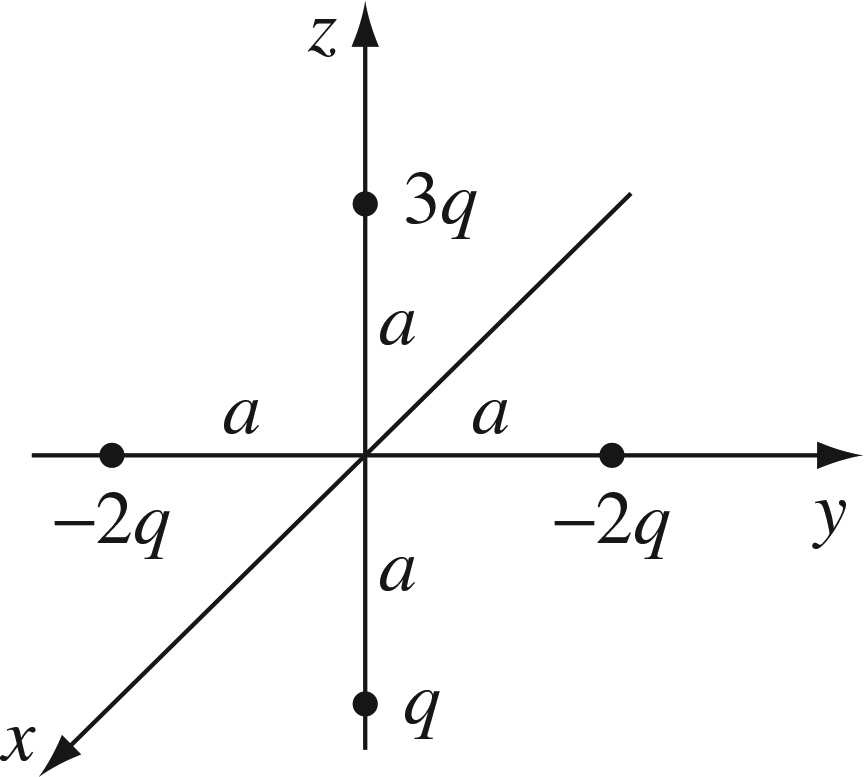
\includegraphics[width=0.225\textwidth]{figures/3_31.jpg} \hspace{1cm}
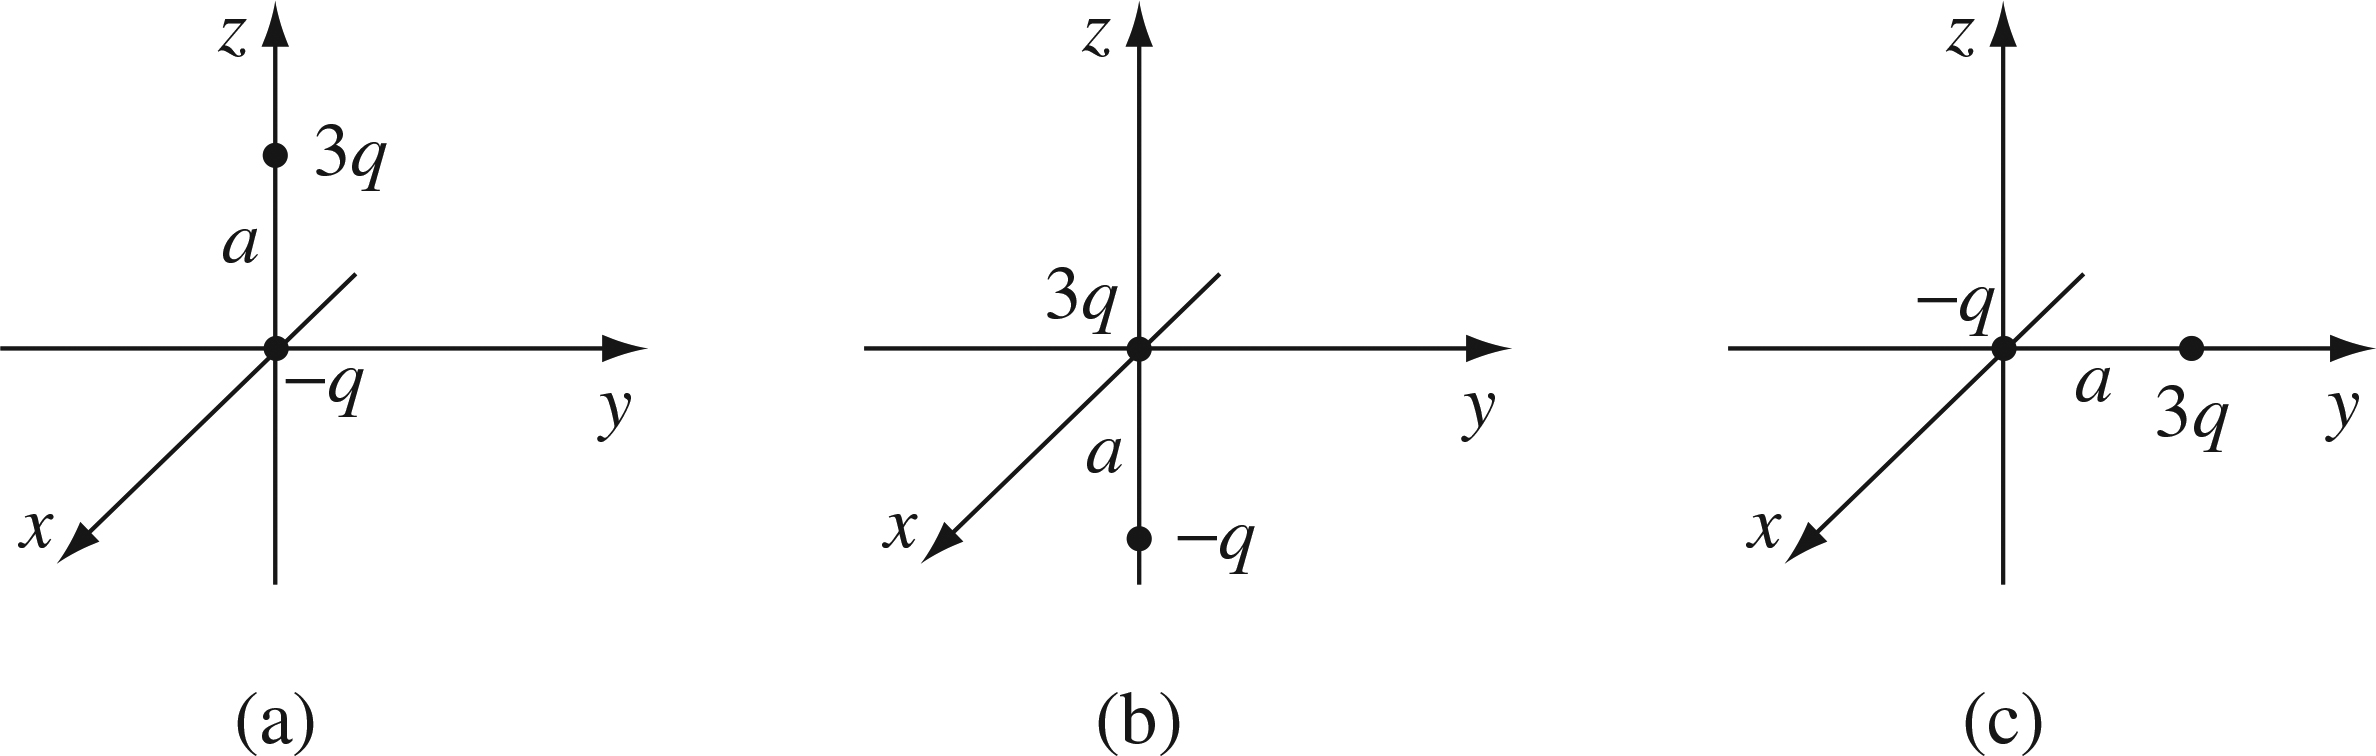
\includegraphics[width=0.65\textwidth]{figures/3_35.jpg}
\caption{\label{fig:dipoles} (Left) An arrangement of four charges near the origin.  (Right, a-c) An arrangement of two charges near the origin, oriented three different ways.}
\end{figure}

\begin{itemize}
\item (a) The far-left configuration has a total charge (monopole moment) of zero.  The monopole term in the multipole expansion vanishes and we're left with the dipole moment.  The y-component of the dipole moment vanishes by symmetry and we have
\begin{equation}
\mathbf{p} = (3qa - qa)\hat{\mathbf{z}} = 2qa\hat{\mathbf{z}}
\end{equation}
This makes the potential in the far-field
\begin{equation}
V(r,\theta) = \frac{1}{4\pi\epsilon_0}\frac{\mathbf{p} \cdot \hat{\mathbf{r}}}{r^2} = \frac{1}{4\pi\epsilon_0}\frac{2qa\cos\theta}{r^2}
\end{equation}
\item For the rest, note that each configuration has a monopole moment of $2q$.  The dipole moments of the three configurations, from left to right, are $3qa\hat{\mathbf{z}}$, $qa\hat{\mathbf{z}}$, and $3qa\hat{\mathbf{y}}$.  The dipole moments are the sum of charge times distance vector (Eq. 3.100 in Ch. 3).  The far-field potentials are then:
\begin{itemize}
\item Configuration a ($\hat{z} \cdot \hat{r} = \cos\theta$):
\begin{equation}
V(r,\theta) = \frac{1}{4\pi\epsilon_0}\left( \frac{2q}{r} + \frac{3qa\cos\theta}{r^2}\right)
\end{equation}
\item Configuration b ($\hat{z} \cdot \hat{r} = \cos\theta$):
\begin{equation}
V(r,\theta) = \frac{1}{4\pi\epsilon_0}\left( \frac{2q}{r} + \frac{qa\cos\theta}{r^2}\right)
\end{equation}
\item Configuration c ($\hat{y} \cdot \hat{r} = \sin\theta\sin\phi$):
\begin{equation}
V(r,\theta) = \frac{1}{4\pi\epsilon_0}\left( \frac{2q}{r} + \frac{3qa\sin\theta\sin\phi}{r^2}\right)
\end{equation}
\end{itemize}
\end{itemize}

\end{enumerate}

\end{document}
